\documentclass[tikz,border=8pt]{standalone}
\usepackage[T1]{fontenc}
\usepackage[scaled=0.92]{sourcesanspro}
\renewcommand{\familydefault}{\sfdefault}
\usetikzlibrary{arrows.meta,positioning,calc,backgrounds,shapes.geometric,shapes.arrows}
\begin{document}
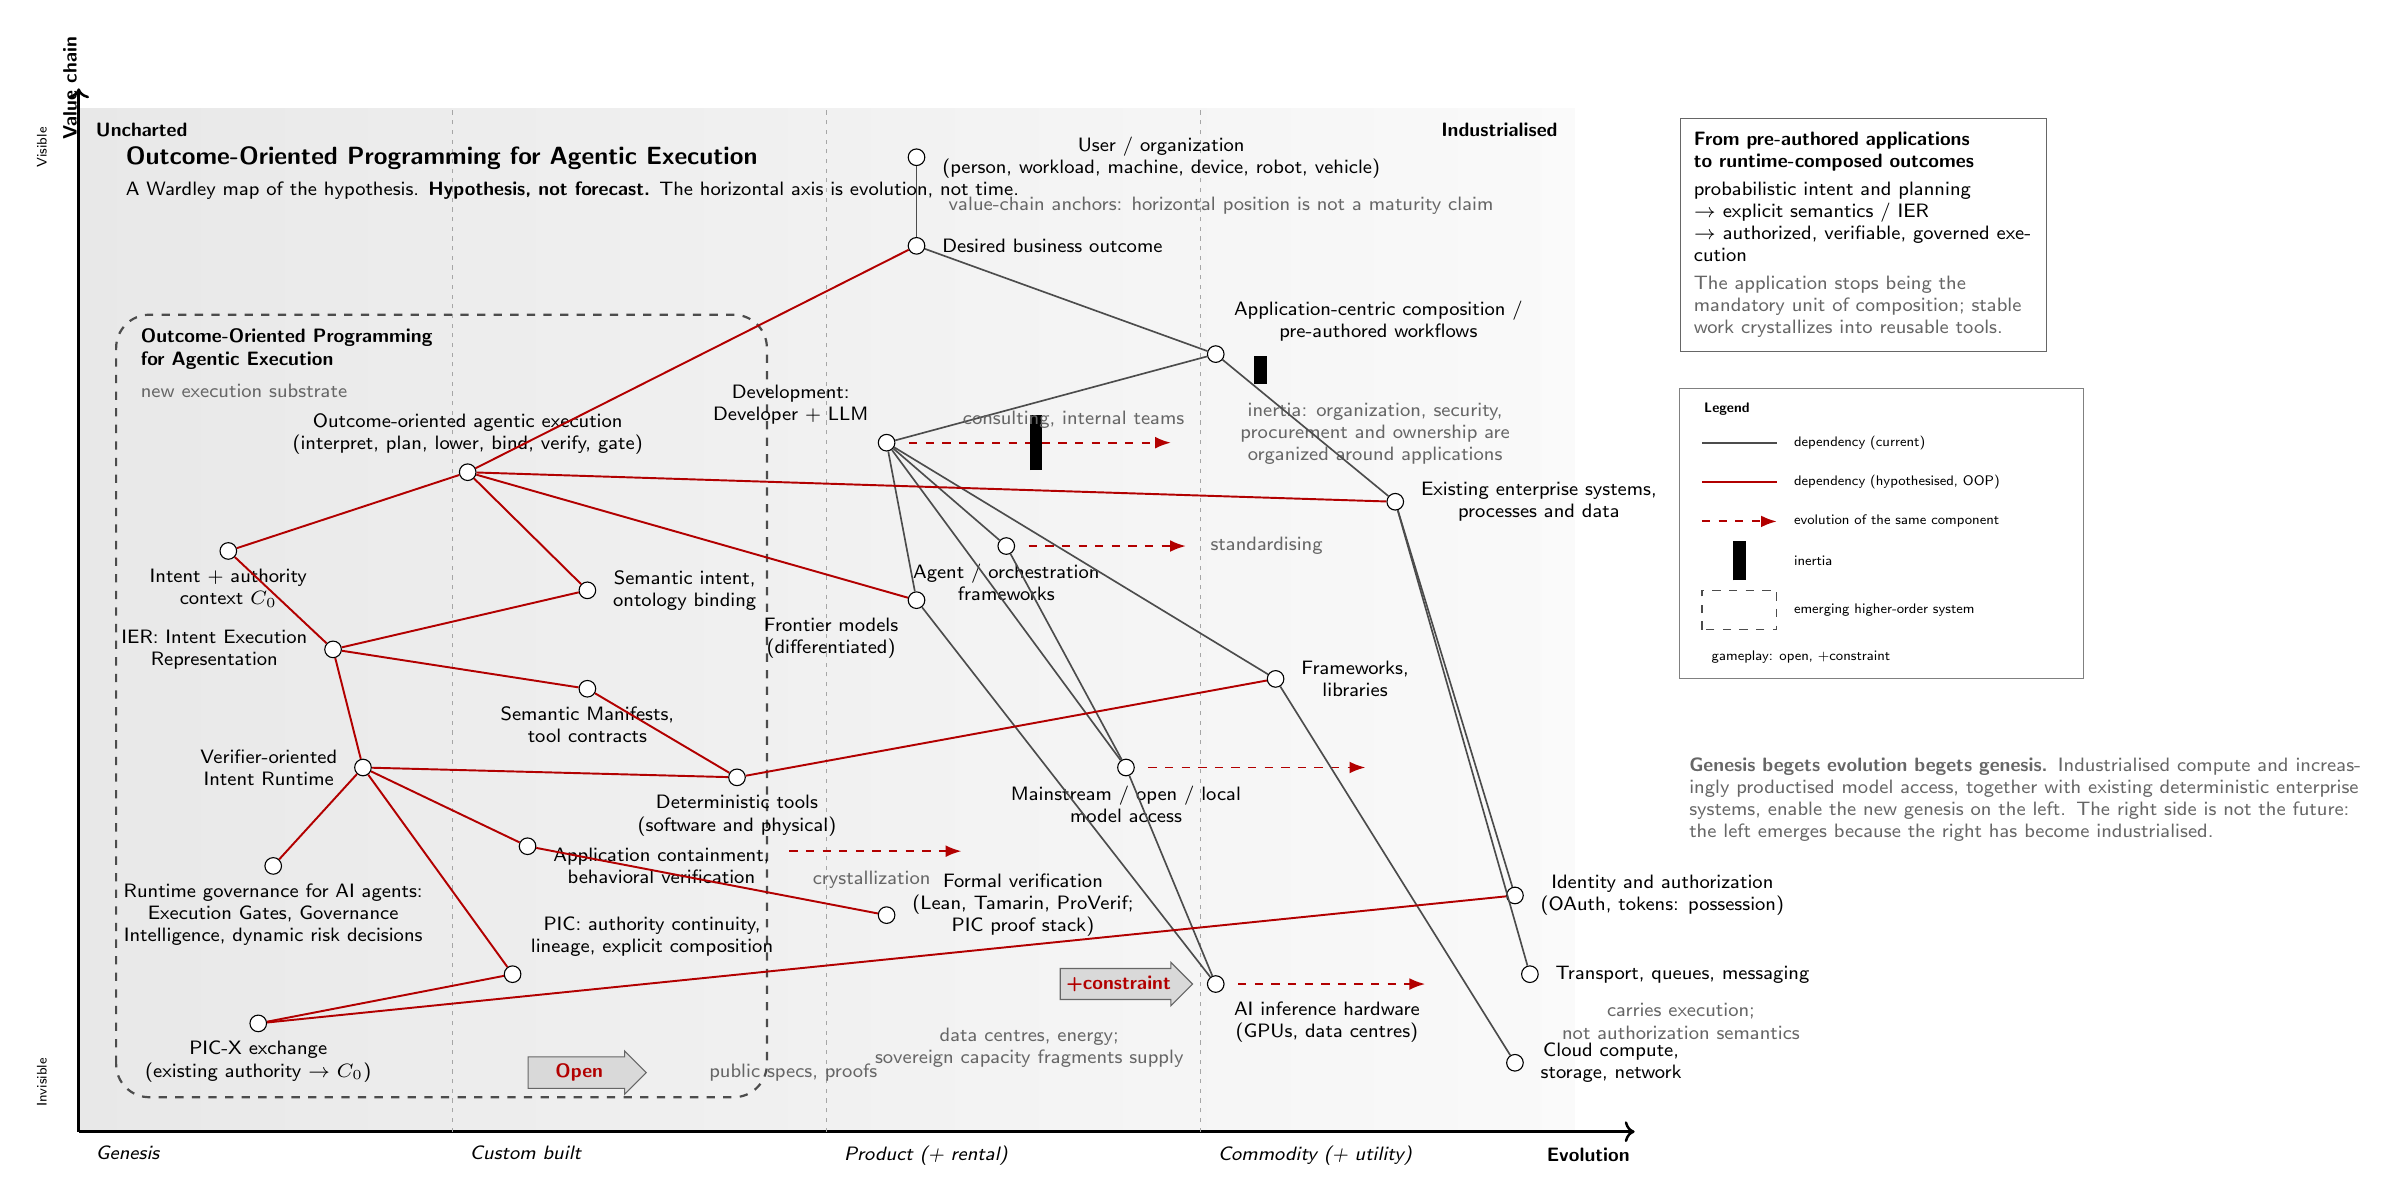
\begin{tikzpicture}[x=1.9cm,y=1.25cm,
  comp/.style={circle, draw=black, fill=white, minimum size=6pt, inner sep=0pt},
  lbl/.style={font=\scriptsize, align=center, inner sep=1pt},
  dep/.style={draw=black!70, line width=0.6pt},
  hyp/.style={draw=red!70!black, line width=0.7pt},
  evo/.style={->, >={Latex[length=2mm]}, red!70!black, dashed, line width=0.7pt},
  inertia/.style={line width=4.5pt, black},
  gp/.style={single arrow, draw=black!60, fill=black!15, minimum height=1.5cm, minimum width=0.55cm, single arrow head extend=2pt, font=\scriptsize\bfseries, text=red!70!black, inner sep=2pt},
  note/.style={font=\scriptsize, text=black!60, align=center}
]
% ---------------- canvas ----------------
\fill[left color=black!9, right color=black!2] (0,0) rectangle (10,10.4);
\draw[->, line width=0.9pt] (0,0) -- (10.4,0) node[below left=2pt and -2pt, font=\scriptsize\bfseries] {Evolution};
\draw[->, line width=0.9pt] (0,0) -- (0,10.6) node[left=1pt, rotate=90, anchor=south, font=\scriptsize\bfseries, yshift=-4pt] {Value chain};
\foreach \x in {2.5,5,7.5}{\draw[black!35, dash pattern=on 1.5pt off 2pt] (\x,0) -- (\x,10.4);}
\node[font=\scriptsize\itshape, anchor=north west] at (0.05,-0.05) {Genesis};
\node[font=\scriptsize\itshape, anchor=north west] at (2.55,-0.05) {Custom built};
\node[font=\scriptsize\itshape, anchor=north west] at (5.05,-0.05) {Product (+ rental)};
\node[font=\scriptsize\itshape, anchor=north west] at (7.55,-0.05) {Commodity (+ utility)};
\node[font=\scriptsize\bfseries, anchor=north west] at (0.05,10.35) {Uncharted};
\node[font=\scriptsize\bfseries, anchor=north east] at (9.95,10.35) {Industrialised};
\node[font=\tiny, rotate=90, anchor=south] at (-0.15,10.0) {Visible};
\node[font=\tiny, rotate=90, anchor=south] at (-0.15,0.5) {Invisible};
\node[font=\small\bfseries, anchor=north west] at (0.25,10.1) {Outcome-Oriented Programming for Agentic Execution};
\node[font=\scriptsize, anchor=north west] at (0.25,9.75) {A Wardley map of the hypothesis. \textbf{Hypothesis, not forecast.} The horizontal axis is evolution, not time.};

% ---------------- emerging higher-order system (dashed enclosure) ----------------
\draw[black!70, dashed, line width=0.8pt, rounded corners=12pt] (0.25,0.35) rectangle (4.6,8.3);
\node[font=\scriptsize\bfseries, anchor=north west, align=left] at (0.35,8.25) {Outcome-Oriented Programming\\for Agentic Execution};
\node[note, anchor=north west] at (0.35,7.7) {new execution substrate};

% ---------------- anchors ----------------
\node[comp] (user) at (5.6,9.9) {};
\node[lbl, anchor=west] at (5.75,9.9) {User / organization\\(person, workload, machine, device, robot, vehicle)};
\node[note, anchor=north west] at (5.75,9.6) {value-chain anchors: horizontal position is not a maturity claim};
\node[comp] (outcome) at (5.6,9.0) {};
\node[lbl, anchor=west] at (5.75,9.0) {Desired business outcome};
\draw[dep] (user) -- (outcome);

% ---------------- incumbent: application-centric composition ----------------
\node[comp] (app) at (7.6,7.9) {};
\node[lbl, anchor=south west] at (7.7,8.0) {Application-centric composition /\\pre-authored workflows};
\draw[dep] (outcome) -- (app);
\draw[inertia] (7.9,7.6) -- (7.9,7.88);
\node[note, anchor=north west] at (7.7,7.5) {inertia: organization, security,\\procurement and ownership are\\organized around applications};

\node[comp] (dev) at (5.4,7.0) {};
\node[lbl, anchor=south east] at (5.3,7.15) {Development:\\Developer + LLM};
\draw[dep] (app) -- (dev);
\draw[evo] (5.55,7.0) -- (7.3,7.0);
\draw[inertia] (6.4,6.72) -- (6.4,7.28);
\node[note, anchor=south] at (6.65,7.05) {consulting, internal teams};

\node[comp] (agentfw) at (6.2,5.95) {};
\node[lbl, anchor=north] at (6.2,5.8) {Agent / orchestration\\frameworks};
\draw[dep] (dev) -- (agentfw);
\draw[evo] (6.35,5.95) -- (7.4,5.95);
\node[note, anchor=west] at (7.5,5.95) {standardising};

\node[comp] (enterprise) at (8.8,6.4) {};
\node[lbl, anchor=west] at (8.95,6.4) {Existing enterprise systems,\\processes and data};
\draw[dep] (app) -- (enterprise);

\node[comp] (frontier) at (5.6,5.4) {};
\node[lbl, anchor=north east] at (5.5,5.25) {Frontier models\\(differentiated)};
\draw[dep] (dev) -- (frontier);

\node[comp] (openm) at (7.0,3.7) {};
\node[lbl, anchor=north] at (7.0,3.55) {Mainstream / open / local\\model access};
\draw[evo] (7.15,3.7) -- (8.6,3.7);
\draw[dep] (dev) -- (openm);
\draw[dep] (agentfw) -- (openm);

\node[comp] (libs) at (8.0,4.6) {};
\node[lbl, anchor=west] at (8.15,4.6) {Frameworks,\\libraries};
\draw[dep] (dev) -- (libs);

\node[comp] (oauth) at (9.6,2.4) {};
\node[lbl, anchor=west] at (9.75,2.4) {Identity and authorization\\(OAuth, tokens: possession)};
\draw[dep] (enterprise) -- (oauth);

\node[comp] (transport) at (9.7,1.6) {};
\node[lbl, anchor=west] at (9.85,1.6) {Transport, queues, messaging};
\node[note, anchor=north west] at (9.85,1.4) {carries execution;\\not authorization semantics};
\draw[dep] (enterprise) -- (transport);

\node[comp] (gpu) at (7.6,1.5) {};
\node[lbl, anchor=north west] at (7.7,1.35) {AI inference hardware\\(GPUs, data centres)};
\draw[dep] (frontier) -- (gpu);
\draw[dep] (openm) -- (gpu);
\draw[evo] (7.75,1.5) -- (9.0,1.5);
\node[gp, anchor=east] at (7.45,1.5) {+constraint};
\node[note, anchor=north east] at (7.45,1.15) {data centres, energy;\\sovereign capacity fragments supply};

\node[comp] (compute) at (9.6,0.7) {};
\node[lbl, anchor=west] at (9.75,0.7) {Cloud compute,\\storage, network};
\draw[dep] (libs) -- (compute);

% ---------------- the new genesis: agentic execution and its substrate ----------------
\node[comp] (agentic) at (2.6,6.7) {};
\node[lbl, anchor=south] at (2.6,6.85) {Outcome-oriented agentic execution\\(interpret, plan, lower, bind, verify, gate)};
\draw[hyp] (outcome) -- (agentic);
\draw[hyp] (agentic) -- (frontier);
\draw[hyp] (agentic) -- (enterprise);

\node[comp] (intent) at (1.0,5.9) {};
\node[lbl, anchor=north] at (1.0,5.75) {Intent + authority\\context $C_0$};
\draw[hyp] (agentic) -- (intent);

\node[comp] (onto) at (3.4,5.5) {};
\node[lbl, anchor=west] at (3.55,5.5) {Semantic intent,\\ontology binding};
\draw[hyp] (agentic) -- (onto);

\node[comp] (ier) at (1.7,4.9) {};
\node[lbl, anchor=east] at (1.55,4.9) {IER: Intent Execution\\Representation};
\draw[hyp] (intent) -- (ier);
\draw[hyp] (onto) -- (ier);

\node[comp] (manifests) at (3.4,4.5) {};
\node[lbl, anchor=north] at (3.4,4.35) {Semantic Manifests,\\tool contracts};
\draw[hyp] (ier) -- (manifests);

\node[comp] (runtime) at (1.9,3.7) {};
\node[lbl, anchor=east] at (1.75,3.7) {Verifier-oriented\\Intent Runtime};
\draw[hyp] (ier) -- (runtime);

\node[comp] (tools) at (4.4,3.6) {};
\node[lbl, anchor=north] at (4.4,3.45) {Deterministic tools\\(software and physical)};
\draw[hyp] (manifests) -- (tools);
\draw[hyp] (runtime) -- (tools);
\draw[evo] (4.75,2.85) -- (5.9,2.85);
\node[note, anchor=north] at (5.3,2.75) {crystallization};
\draw[hyp] (tools) -- (libs);

\node[comp] (contain) at (3.0,2.9) {};
\node[lbl, anchor=west] at (3.15,2.7) {Application containment,\\behavioral verification};
\draw[hyp] (runtime) -- (contain);

\node[comp] (formal) at (5.4,2.2) {};
\node[lbl, anchor=west] at (5.55,2.3) {Formal verification\\(Lean, Tamarin, ProVerif;\\PIC proof stack)};
\draw[hyp] (contain) -- (formal);

\node[comp] (gates) at (1.3,2.7) {};
\node[lbl, anchor=north] at (1.3,2.55) {Runtime governance for AI agents:\\Execution Gates, Governance\\Intelligence, dynamic risk decisions};
\draw[hyp] (runtime) -- (gates);

\node[comp] (pic) at (2.9,1.6) {};
\node[lbl, anchor=south west] at (3.0,1.75) {PIC: authority continuity,\\lineage, explicit composition};
\draw[hyp] (runtime) -- (pic);

\node[comp] (picx) at (1.2,1.1) {};
\node[lbl, anchor=north] at (1.2,0.95) {PIC-X exchange\\(existing authority $\rightarrow C_0$)};
\draw[hyp] (pic) -- (picx);
\draw[hyp] (picx) -- (oauth);
\node[gp, anchor=west] at (3.0,0.6) {Open};
\node[note, anchor=west] at (4.15,0.6) {public specs, proofs};

% ---------------- core message (outside canvas) ----------------
\node[draw=black!60, fill=white, align=left, font=\scriptsize, anchor=north west, inner sep=5pt, text width=4.3cm] at (10.7,10.3)
 {\textbf{From pre-authored applications}\\\textbf{to runtime-composed outcomes}\\[2pt]
  probabilistic intent and planning\\$\rightarrow$ explicit semantics / IER\\$\rightarrow$ authorized, verifiable, governed execution\\[2pt]
  {\color{black!60}The application stops being the mandatory unit of composition; stable work crystallizes into reusable tools.}};

% ---------------- legend (outside canvas) ----------------
\begin{scope}[shift={(10.7,4.6)}]
\fill[white, draw=black!50] (0,0) rectangle (2.7,2.95);
\node[font=\tiny\bfseries, anchor=north west] at (0.1,2.9) {Legend};
\draw[dep] (0.15,2.4) -- (0.65,2.4); \node[font=\tiny, anchor=west] at (0.7,2.4) {dependency (current)};
\draw[hyp] (0.15,2.0) -- (0.65,2.0); \node[font=\tiny, anchor=west] at (0.7,2.0) {dependency (hypothesised, OOP)};
\draw[evo] (0.15,1.6) -- (0.65,1.6); \node[font=\tiny, anchor=west] at (0.7,1.6) {evolution of the same component};
\draw[inertia] (0.4,1.0) -- (0.4,1.4); \node[font=\tiny, anchor=west] at (0.7,1.2) {inertia};
\draw[black!70, dashed] (0.15,0.5) rectangle (0.65,0.9); \node[font=\tiny, anchor=west] at (0.7,0.7) {emerging higher-order system};
\node[font=\tiny, anchor=west] at (0.15,0.22) {gameplay: open, +constraint};
\end{scope}

% ---------------- the Wardley pattern (below the canvas) ----------------
\node[note, anchor=north west, text width=8.6cm, align=left] at (10.7,3.9) {\textbf{Genesis begets evolution begets genesis.} Industrialised compute and increasingly productised model access, together with existing deterministic enterprise systems, enable the new genesis on the left. The right side is not the future: the left emerges because the right has become industrialised.};
\end{tikzpicture}
\end{document}
